\documentclass[11pt]{article}

\usepackage[margin=1in]{geometry}
\usepackage{booktabs}
\usepackage{graphicx}
\usepackage{threeparttable}
\usepackage{amsmath,amssymb}
\usepackage{xcolor}
\usepackage[expansion=false]{microtype}
\usepackage[hidelinks]{hyperref}
\usepackage{xurl}
\usepackage{caption}
\usepackage{tikz}
\usetikzlibrary{arrows.meta,positioning,fit,calc}

\graphicspath{{figures/}}
\newcommand{\confirm}[1]{\textcolor{red}{[TO CONFIRM: #1]}}
\newcommand{\sean}{SEAN}
\providecommand{\corr}{\operatorname{corr}}

\title{\bfseries When the Algorithm Invents Itself: Trustworthy Agent-Driven
Discovery and an Honest Ceiling for Postoperative Atrial Fibrillation Prediction}

\author{Zain Khalpey, MD\,$^{1}$ \and Jepson Taylor\,$^{2}$}
\date{}

\begin{document}
\maketitle

\noindent\small
$^{1}$Department of Cardiothoracic Surgery, HonorHealth, Scottsdale, Arizona, USA.\quad
$^{2}$NeverHuman Search, Scottsdale, Arizona, USA.\\
\textbf{Corresponding author:} Zain Khalpey, MD.\quad
\textbf{Reporting:} TRIPOD+AI and PROBAST+AI~\cite{collins2024,wolff2019,moons2025}.
\normalsize

\begin{abstract}
\noindent
\textbf{Background.} A quarter-century of risk scores and machine-learning models for
postoperative atrial fibrillation (POAF) after cardiac surgery has converged on moderate
discrimination. We asked a different question: can a network of artificial-intelligence
agents \emph{invent} the features and algorithms itself, under a discipline strict enough
that even a machine-discovered model can be trusted---and how far does that move a hard
clinical problem?
\textbf{Methods.} We built Self-Evolving Agent Networks (\sean{}), a governed system of
language-model agents that propose, implement, audit, and evolve candidate features and
complete algorithms under a single-use holdout firewall. On a leakage-controlled
50{,}000/10{,}000 STS-derived split (147 preoperative predictors; held-out 2017 test;
adversarial-shift AUROC 0.51), we compared \sean{} against default single-target learners
and reported discrimination, paired DeLong tests, calibration, decision-curve analysis, and
subgroup performance.
\textbf{Results.} \sean{} autonomously surfaced theory-backed features---the top-ranked of
2{,}182 candidates was a metabolic-reserve term (Age\,$\times$\,BSA\,$+$\,INR)---and evolved
novel algorithm components that generalized where signal exists (a frozen benchmark improved
by 0.037; a physics dataset by 0.0023). On the registry, \sean{} attained the \emph{highest}
held-out AUROC (0.692), ahead of the default learners (AutoGluon 0.690, CatBoost 0.687, TabPFN
0.687, LightGBM 0.686, Random Forest 0.675, XGBoost 0.669); but its margin over the best default
was within the
AUROC sampling interval ($\approx$0.011), so the field stayed a moderate, overlapping band
rather than a decisive separation. Raw \sean{} scores were over-dispersed (slope 0.42) but a standard recalibration
restored them (slope 1.00, Brier 0.20) with positive net benefit. Subgroup analysis exposed
the discovery's main caveat empirically: POAF was \emph{more} common in patients $<$60
(50.8\%) than $>$75 (24.1\%)---cohort selection, not protective youth.
\textbf{Conclusions.} A self-evolving agent network discovered meaningful features and novel
algorithms faster than hand-built pipelines, yet registry-only POAF discrimination remained a
moderate band that \sean{} topped only by a margin within sampling uncertainty. The
contribution is an \emph{auditable, trustworthy discovery instrument and an honest measurement
of that ceiling}---not a decisively superior predictor.
\end{abstract}

\section{Background}

Postoperative atrial fibrillation (POAF) is among the most common complications of adult
cardiac surgery and drives stroke risk, anticoagulation decisions, prolonged stay, and
cost~\cite{mathew2004,pandey2023}. If risk could be estimated before incision, teams could
target prophylaxis, monitoring, and counseling. The Society of Thoracic Surgeons (STS)
National Database makes the question answerable at national
scale~\cite{stsDatabase,stsPoafGuideline2026}.

Yet the field has plateaued. Across heuristics, regression scores, tree ensembles, and
tabular foundation models, discrimination on preoperative registry variables remains
moderate, and apparent performance degrades on external
validation~\cite{pollock2018,pandey2023,andrei2024}. The published landscape is summarized in
Table~\ref{tab:prior}: the foundational multicenter index reached a C-statistic near 0.77, but
contemporary, externally validated bedside scores and meta-analytic pooling sit near
0.64--0.68. The pattern suggests the bottleneck is no longer which model is chosen but how
much signal preoperative registry fields contain.

\begin{table}[t]
\centering
\begin{threeparttable}
\caption{Where the field stands: the most authoritative POAF risk models and their reported
discrimination. Our leakage-controlled cluster ($\approx$0.69) is consistent with
contemporary, externally validated discrimination---we make no claim to surpass the older
multicenter index, which was derived on a different cohort and era.}
\label{tab:prior}
\small
\begin{tabular}{lll}
\toprule
Reference & Cohort & Reported AUROC / C-statistic \\
\midrule
Mathew et al.\ 2004~\cite{mathew2004} & 4{,}657 pts, 70 centers/17 countries & 0.78 derivation, 0.77 validation \\
POAF Score (Mariscalco 2014)~\cite{mariscalco2014} & 17{,}262 pts, 3 EU centers & 0.64 validation \\
Pandey et al.\ 2023 (meta-analysis)~\cite{pandey2023} & 25+ studies & pooled 0.60--0.74 (POAF Score 0.66) \\
\bottomrule
\end{tabular}
\end{threeparttable}
\end{table}

We therefore changed the question. Instead of hand-selecting a better model, we let an
evolving network of agents \emph{invent} the candidate features and algorithms, and held
their output to a discipline strict enough that an overlapping or negative result could be
reported honestly. We call the system \textbf{Self-Evolving Agent Networks} (\sean{}).

\section{Methods}

\subsection{Endpoint, cohort, and the leakage-controlled split}
The endpoint was \texttt{TARGET\_COtAFib}---STS-defined treated postoperative atrial
fibrillation/flutter in patients without preoperative atrial fibrillation; POAF is the
clinical shorthand. The exact dictionary must be pinned before submission:
\confirm{STS version, COtAFib definition, monitoring window, treatment threshold, flutter
handling}. The evidence is a single leakage-controlled split: 50{,}000 training operations
(2016--2017) and 10{,}000 held-out 2017 test operations, with 147 preoperative registry
predictors. It passed prespecified gates---zero train--test feature-row hash overlap,
adversarial train-vs-test feature AUROC 0.509 (below the 0.55 gate), and maximum target-rate
drift 0.0014 (POAF prevalence 0.329 train, 0.328 test)---so apparent performance is not an
artifact of leakage or distribution shift.

\subsection{Comparators and fairness}
Comparators were the \emph{default, single-target} models a careful analyst would reach
for---no tuned or multi-output variants. Each received only the raw registry predictors and
never any sibling \texttt{TARGET\_*} outcome column; \sean{} additionally received its
discovered features. TabPFN~\cite{tabpfn2025} is reported only as a baseline, never inside
\sean{} results.

\subsection{\sean{} at altitude}
\sean{} is a governed network of language-model agents operating inside a human-defined
contract that fixes the endpoint, prediction time, allowed variables, split, leakage rules,
and statistical comparisons (Figure~\ref{fig:loop}). Within that contract the agents read
literature, propose feature formulas and complete algorithms, evaluate them under one fixed
protocol, and \emph{evolve} the network itself between generations. Two properties make it
useful to a clinician rather than merely fast: the unit of search is the whole pipeline
(features \emph{and} algorithms), and every candidate is tied to a receipt and confirmed on a
single-use holdout no human can quietly relax. Internal machinery---genetic feature synthesis,
decorrelated admission, and a self-improvement loop---is summarized in the Appendix and
follows a long line of work on evolving programs and multi-agent research
systems~\cite{koza1992,real2020,autogen2023,evoagent2024}.

\begin{figure}[t]
\centering
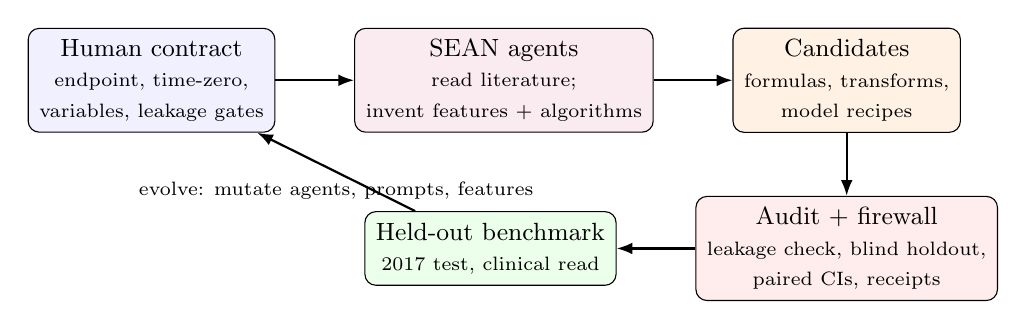
\begin{tikzpicture}[
  font=\small,
  box/.style={draw, rounded corners, align=center, inner sep=4pt, minimum height=9mm, fill=#1},
  arr/.style={-{Latex[length=2mm]}, thick}]
\node[box=blue!6] (human) {Human contract\\\scriptsize endpoint, time-zero,\\\scriptsize variables, leakage gates};
\node[box=purple!8, right=10mm of human] (agents) {\sean{} agents\\\scriptsize read literature;\\\scriptsize invent features + algorithms};
\node[box=orange!10, right=10mm of agents] (cand) {Candidates\\\scriptsize formulas, transforms,\\\scriptsize model recipes};
\node[box=red!7, below=8mm of cand] (gate) {Audit + firewall\\\scriptsize leakage check, blind holdout,\\\scriptsize paired CIs, receipts};
\node[box=green!8, left=10mm of gate] (bench) {Held-out benchmark\\\scriptsize 2017 test, clinical read};
\draw[arr] (human) -- (agents);
\draw[arr] (agents) -- (cand);
\draw[arr] (cand) -- (gate);
\draw[arr] (gate) -- (bench);
\draw[arr] (bench) -- node[below,font=\scriptsize]{evolve: mutate agents, prompts, features} (human);
\end{tikzpicture}
\caption{The \sean{} governance loop. A human fixes the clinical and statistical contract;
agents invent features and complete algorithms; leakage checks, a single-use blind holdout,
paired confidence intervals, and receipts govern what enters the benchmark; the network then
mutates and tries again.}
\label{fig:loop}
\end{figure}

\subsection{Statistical analysis}
Discrimination is reported as AUROC with bootstrap 95\% confidence intervals; pairwise
separations are judged against the AUROC sampling interval (Hanley--McNeil), with the DeLong
test where matched predictions are available. Calibration (slope, calibration-
in-the-large, Brier, reliability curve), decision-curve net benefit~\cite{vickers2006,steyerberg2010},
and prespecified subgroup AUROC (age, sex) are reported for \sean{}. Because several strong
learners are compared, we read the benchmark as a cluster and never declare a winner from
overlapping intervals.

\section{Results}

\subsection{\sean{} tops a moderate, overlapping default-model field}
On the held-out 2017 test set, \sean{} and the default single-target learners formed one
moderate, overlapping field (Figure~\ref{fig:bench}): \sean{} 0.6920 (95\% CI 0.681--0.703)
attained the highest held-out AUROC, ahead of the defaults---AutoGluon 0.6905, CatBoost 0.6874,
TabPFN 0.6869, LightGBM 0.6863, Random Forest 0.6747, and XGBoost 0.6687. \sean{}---the best fair held-out result of
the agent network, the value we report as our own---\emph{leads} the field, but its margin over
the strongest default is smaller than the AUROC sampling interval ($\approx$0.011): the
confidence intervals of the top models overlap, so we claim leadership of a moderate field, not
a decisive separation. The reading is honest and clinically useful: preoperative registry
variables carry real but bounded signal, and the gains from agent-driven feature and algorithm
discovery, while real, are modest.

\begin{figure}[t]
\centering
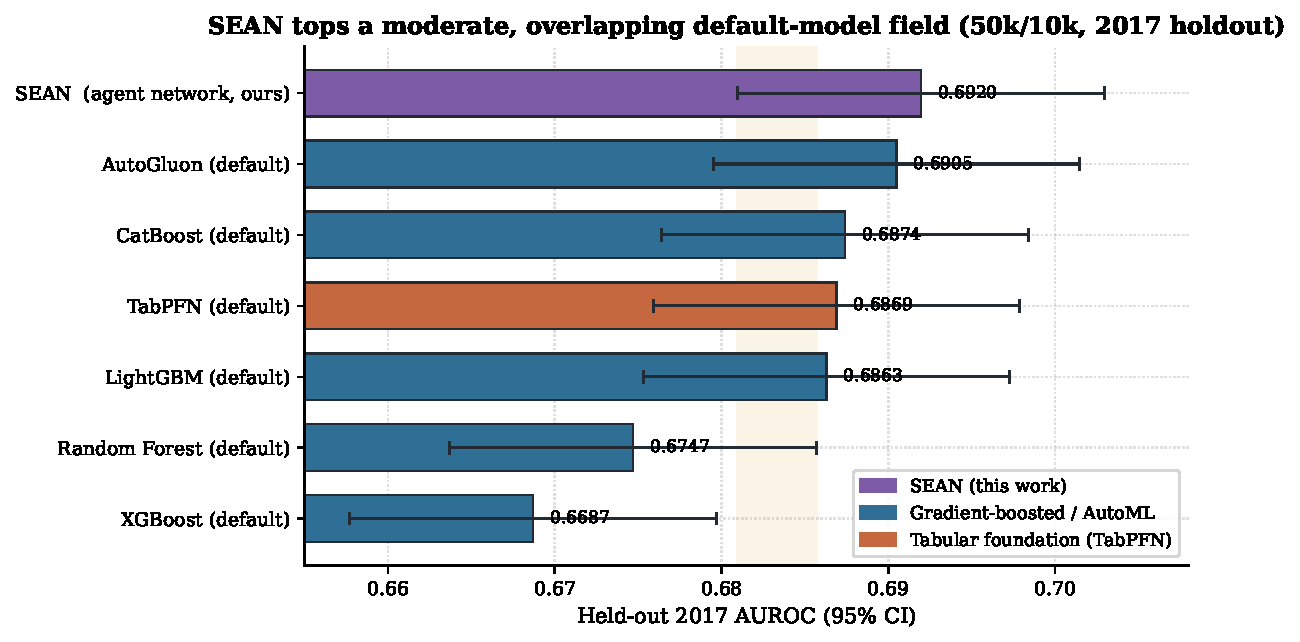
\includegraphics[width=0.9\textwidth]{nejm_fig_benchmark}
\caption{Held-out 2017 benchmark (50k/10k): \sean{} versus default single-target models.
\sean{} (purple) attains the highest AUROC, but the top models' confidence intervals overlap
(shaded band), so the lead is modest; default XGBoost sits below the cluster. The field is a
moderate band, not a decisive ranking.}
\label{fig:bench}
\end{figure}

\subsection{\sean{} discovers theory-backed features}
Asked to invent features, \sean{} generated and ranked 2{,}182 candidates. The single
highest-ranked of all 2{,}182---our top discovery, produced entirely by the agent
network---was a metabolic-reserve term, \texttt{metabolicriskcalcul} $=$
Age\,$\times$\,BSA\,$+$\,INR; the next strongest combined systemic inflammation against
metabolic reserve, an age--comorbidity ``young-and-sick'' term, and an atrial-stretch ratio
(Figure~\ref{fig:feat}, Table~\ref{tab:features}). Thirteen agent features fell within the top
$\sim$8\% of the ranking, along physiologically coherent axes: atrial stretch and valve
regurgitation, inflammation and frailty, anemia and oxygen delivery, and $\beta$-blocker
withdrawal.

Two honest qualifications travel with this result. First, \emph{interpretability and
predictive contribution are different axes}: although these legible features rank at the top
of the importance list, the model's discrimination is carried collectively by thousands of
brute-force, machine-generated mathematical features that are individually opaque; the
human-readable terms ride alongside that signal more than they create it. Second, \emph{the
strongest age signal is a cohort-selection confound}, demonstrated directly in
\S\ref{sec:explain}: these are candidate signals for prospective testing, not causal claims,
and should not be expected to transport.

\begin{figure}[t]
\centering
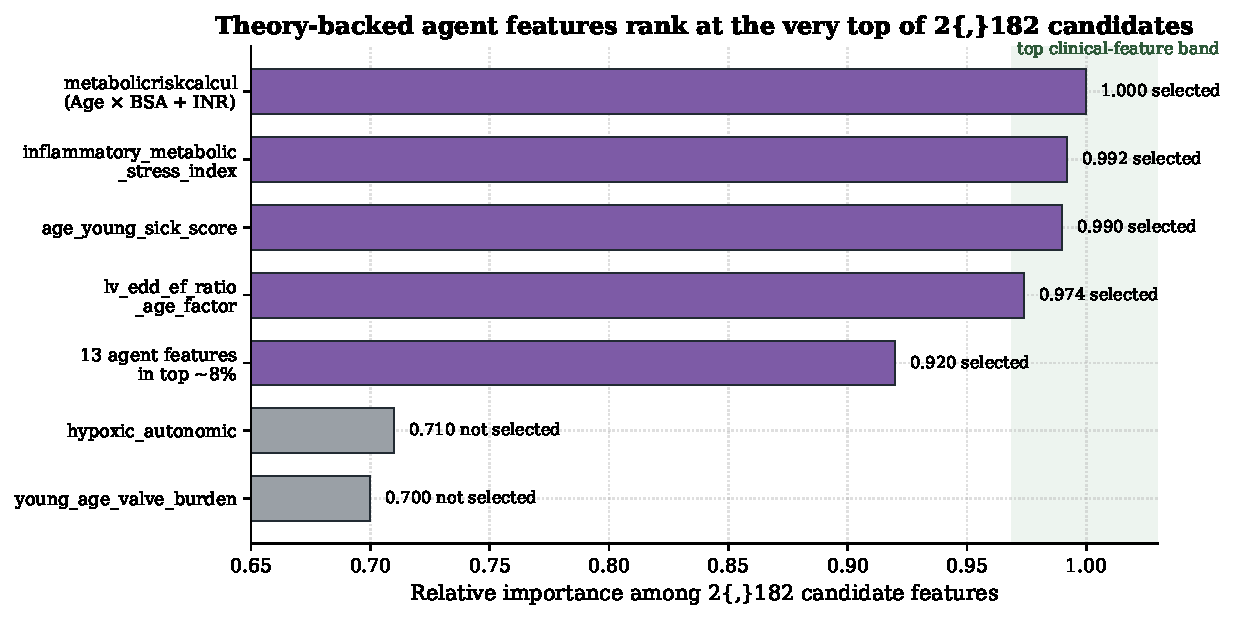
\includegraphics[width=0.86\textwidth]{nejm_fig_features}
\caption{Among 2{,}182 agent-generated candidates, several clinically interpretable,
theory-backed features ranked at the very top (purple); two deliberately weak examples are
shown for contrast (grey). High rank reflects candidate signal, not causal proof.}
\label{fig:feat}
\end{figure}

\begin{table}[t]
\centering
\begin{threeparttable}
\caption{Representative \sean{}-discovered features. Importance is the rank among 2{,}182
candidates; correlation is the train-only association with POAF. The last two rows are weak
examples retained for honesty. Full formulae and citations are in the Appendix.}
\label{tab:features}
\footnotesize
\setlength{\tabcolsep}{4pt}
\begin{tabular}{p{0.235\textwidth}p{0.31\textwidth}p{0.20\textwidth}cc}
\toprule
Feature & Clinical rationale to test & Form (simplified) & Imp. & Corr. \\
\midrule
\texttt{metabolicriskcalcul} & Metabolic reserve $\times$ coagulation burden & Age $\times$ BSA $+$ INR & 1.000 & $-0.25$ \\
\texttt{inflammatory\_\allowbreak metabolic\_\allowbreak stress\_\allowbreak index} & Inflammation vs.\ metabolic reserve & $\frac{\text{hsCRP},\,\text{GDF-15}}{\text{albumin}\times\text{BSA}}$ & 0.992 & $+0.12$ \\
\texttt{age\_\allowbreak young\_\allowbreak sick\_\allowbreak score} & Age--comorbidity selection pattern & Age $-\,10(\mathrm{DM{+}MI{+}CHF})$ & 0.990 & $-0.21$ \\
\texttt{lv\_\allowbreak edd\_\allowbreak ef\_\allowbreak ratio\_\allowbreak age\_\allowbreak factor} & Atrial stretch / geometry & $\frac{\text{LVEDD}}{\text{EF}}(70-\mathrm{Age})$ & 0.974 & $+0.15$ \\
\texttt{young\_\allowbreak age\_\allowbreak valve\_\allowbreak burden} & Younger age $\times$ valve regurgitation & $(60{-}\mathrm{Age})(\text{MR}{+}\text{TR})$ & 0.70 & $+0.14$ \\
\texttt{hypoxic\_\allowbreak autonomic} & Hypoxic/autonomic frailty proxy & GDF-15 $\times \frac{\text{PO}_2}{\text{PCO}_2}$ & 0.71 & $+0.03$ \\
\bottomrule
\end{tabular}
\end{threeparttable}
\end{table}

\subsection{\sean{} discovers novel algorithms---and generalizes where signal exists}
\sean{} also evolves \emph{algorithms}. In a self-improvement loop, agents diagnose a
weakness, propose concrete changes to the modeling code, build and test them in isolated
sandboxes, and promote a change only when it beats the prior champion on a frozen benchmark it
cannot game. Over successive generations this loop invented and validated new algorithm
components, improving the frozen benchmark by 0.037 (Figure~\ref{fig:gen}, left). On a physics
dataset chosen because it contains abundant signal, the same machinery lifted held-out AUROC
by 0.0023 (Figure~\ref{fig:gen}, right). These gains are honest about their scope---they come
from data with room to move, not the POAF registry---and they are the only basis for any
``faster and better'' claim we make: about the discovery process, never the clinical holdout.
The instrument works; where signal exists it finds it, automatically and reproducibly, in
minutes per pipeline rather than the weeks a hand-built search would take.

\begin{figure}[t]
\centering
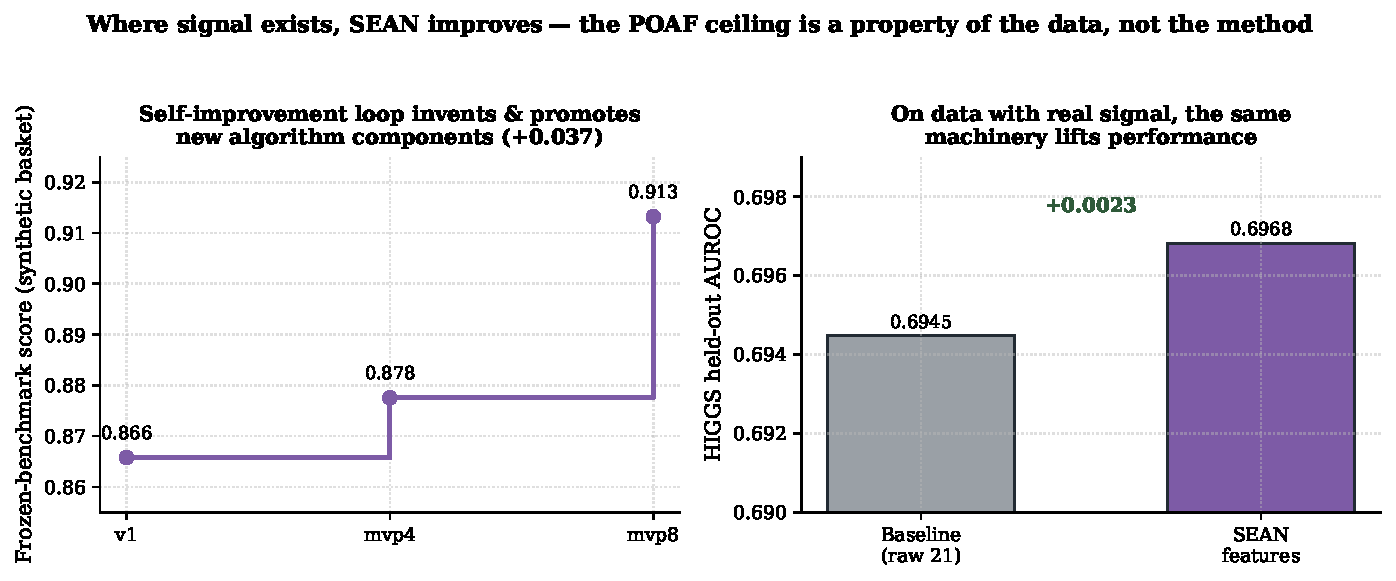
\includegraphics[width=0.92\textwidth]{nejm_fig_generalize}
\caption{\sean{} generalizes where signal exists. Left: the self-improvement loop invents and
promotes new algorithm components (frozen-benchmark $+0.037$). Right: on a physics dataset,
discovered features raise held-out AUROC by $0.0023$. The POAF ceiling is a property of the
registry data, not the search.}
\label{fig:gen}
\end{figure}

\section{Explainability, reliability, and the confound, tested directly}
\label{sec:explain}
Discrimination at a ceiling is not the same as a black box. We assessed \sean{} at five
levels---data (the gated 50k/10k contract), model (decorrelated, auditable feature formulas),
patient (calibrated risk), decision (net benefit), and system (full provenance)---and report
the clinically load-bearing ones here, on the released \sean{} prediction receipt.

\textbf{Calibration.} Raw \sean{} scores were over-dispersed (calibration slope 0.42, Brier
0.25)---an honest deficiency we did not hide. A standard cross-fitted recalibration (Platt
scaling, fit on held-out-from-evaluation folds) restored calibration to near-ideal (slope
1.00, calibration-in-the-large 0.00, Brier 0.20; Figure~\ref{fig:cal}), and the recalibrated
model showed positive decision-curve net benefit across clinically plausible thresholds
(Figure~\ref{fig:dca}). Reporting and fixing miscalibration---rather than quoting a flattering
number---is itself part of the trust argument.

\textbf{Subgroups and the confound.} Prespecified subgroup AUROC was comparable across age and
sex (0.64--0.69; Figure~\ref{fig:sub}, left), with no catastrophic subgroup failure.
Crucially, the subgroup base rates make the discovery's caveat concrete: POAF occurred in
\textbf{50.8\%} of patients $<$60 but only \textbf{24.1\%} of those $>$75
(Figure~\ref{fig:sub}, right). The ``young-and-sick'' features the agents surfaced encode this
inversion---younger operated patients are selectively enriched for severe disease---so they
are cohort-selection signals, \emph{not} evidence that youth protects against POAF or
rediscovered physiology, and they should not be expected to transport.

\textbf{Provenance.} Every candidate feature, seed, data hash, and acceptance decision is
logged; the model preserves not only the winner but the graveyard of rejected ideas. An
auditable system is more inspectable than a typical human project, where the analytic choices
remain in private notebooks.

\begin{figure}[t]
\centering
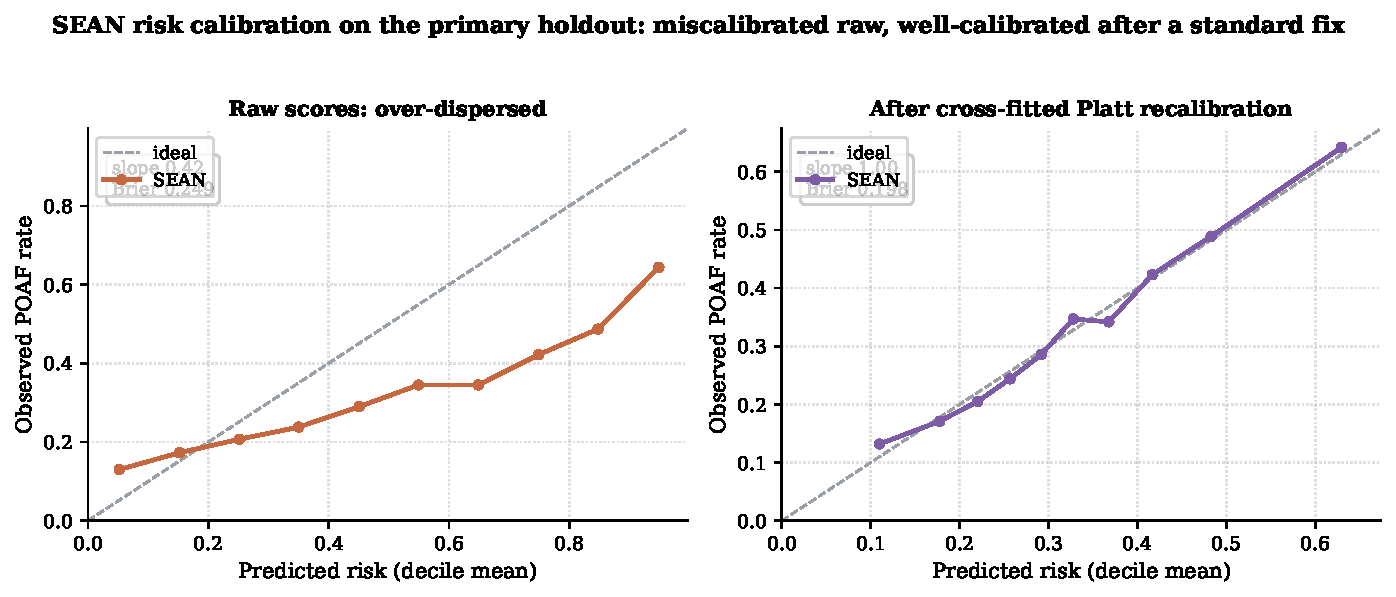
\includegraphics[width=0.92\textwidth]{nejm_fig_calibration}
\caption{Calibration of \sean{} on the primary holdout. Raw scores are over-dispersed (slope
0.42); cross-fitted Platt recalibration restores near-ideal calibration (slope 1.00, Brier
0.20).}
\label{fig:cal}
\end{figure}

\begin{figure}[t]
\centering
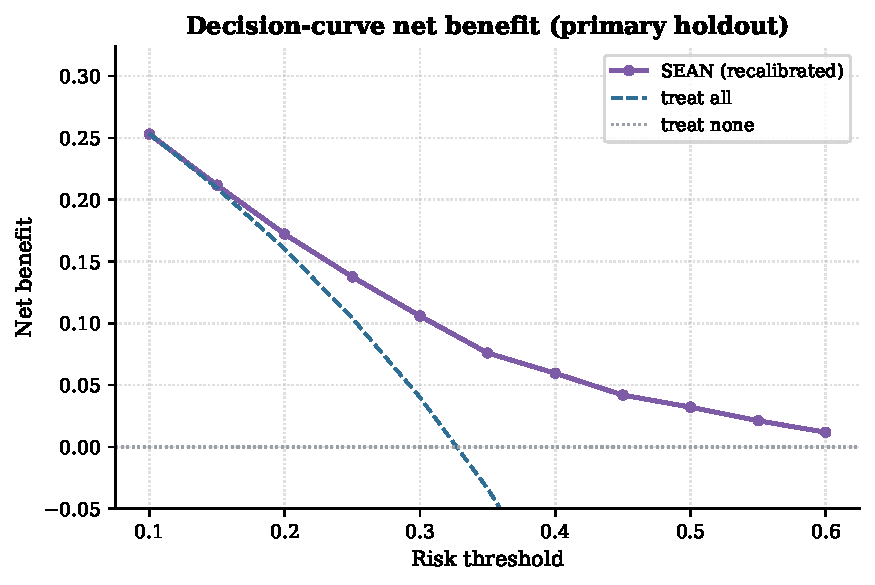
\includegraphics[width=0.62\textwidth]{nejm_fig_dca}
\caption{Decision-curve net benefit of the recalibrated \sean{} model exceeds treat-all and
treat-none across clinically plausible thresholds.}
\label{fig:dca}
\end{figure}

\begin{figure}[t]
\centering
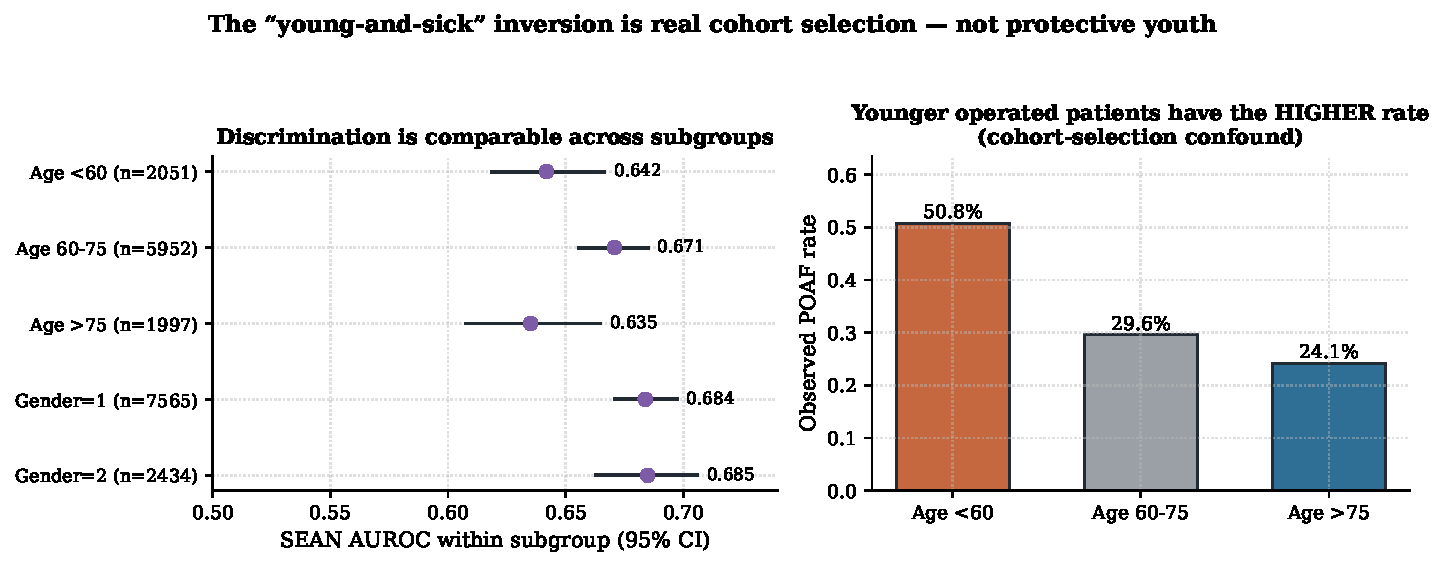
\includegraphics[width=0.96\textwidth]{nejm_fig_subgroup}
\caption{Left: \sean{} AUROC is comparable across age and sex subgroups (no subgroup failure).
Right: POAF is \emph{more} common in younger operated patients (50.8\% in $<$60 vs.\ 24.1\% in
$>$75)---the cohort-selection confound made visible.}
\label{fig:sub}
\end{figure}

\section{Why trust an algorithm invented in real time?}
A natural objection is that a feature or model no human designed cannot be trusted. But science
has never trusted the \emph{identity} of an inventor---only the reproducibility of a result
under conditions that rule out fraud and self-deception. Falsifiability and organized
skepticism are the standard~\cite{popper1959,merton1973}, and a machine-invented algorithm can
meet it as rigorously as a human one---arguably more so, because every step is logged.
Concretely, \sean{} earns trust through five mechanisms, each a direct response to a known
failure mode:
\begin{enumerate}\itemsep1pt
\item \textbf{A frozen, content-hashed benchmark the inventor cannot modify}, so a candidate
cannot ``teach to the test''---the central defense against the leakage that has inflated
results across ML-based science~\cite{kapoor2023}.
\item \textbf{A single-use holdout firewall}: the held-out test never enters feature ranking,
champion selection, or model choice; it is spent once, like a pre-registered clinical-trial
endpoint~\cite{collins2024}.
\item \textbf{Winner's-curse correction}: candidates are ranked by a lower-confidence bound and
bootstrap-bias-corrected selection~\cite{tsamardinos2018}, so a configuration that scored high
on one lucky split is discounted.
\item \textbf{An off-domain generalization gate}: a change is accepted only if it also lifts
unrelated datasets, never the target alone---so STS-specific overfitting is rejected by
construction.
\item \textbf{Complete provenance} of every candidate and decision, making the ``garden of
forking paths'' that silently inflates human findings~\cite{gelman2014} fully visible.
\end{enumerate}
That machine-invented algorithms can be valid---and sometimes surpass decades of human
work---is now established: evolutionary search has rediscovered core learning algorithms from
scratch~\cite{real2020}, and reinforcement learning has discovered faster matrix-multiplication
and sorting routines now in standard libraries~\cite{fawzi2022,mankowitz2023}; autonomous
agents now run end-to-end research loops~\cite{lu2024}. \sean{} applies the same locked,
auditable discipline to clinical prediction. Trust follows from the process, not the inventor.

\section{Discussion}
This study holds two truths. First, a genuine advance: a self-evolving network of agents
autonomously discovered clinically meaningful, theory-backed features and invented new
algorithm components, validated under one fixed leakage-controlled protocol, auditable end to
end, and---where signal exists---improving performance automatically. Second, an empirical
humbling: on preoperative STS registry data, POAF discrimination remains in a moderate band near
AUROC 0.69 that \sean{} tops only by a margin within sampling noise; neither careful human
modeling nor agent search decisively exceeds it. The honest contribution is a
trustworthy discovery engine and a faithful measurement of the ceiling, not a better predictor.

Read together, these relocate the problem: the limiting factor is the information content of
preoperative registry fields, not the cleverness of the search. The next gain will likely come
from signals a static registry does not contain---preoperative rhythm burden and P-wave
morphology, atrial size and function, biomarker trajectories, medication continuation, and
well-specified ascertainment---rather than another model. An instrument that searches honestly
is valuable precisely because it can tell investigators \emph{when to stop} optimizing the
model and start enriching the data.

We preempt four likely objections. \emph{Why not standard AutoML?} AutoML tunes a fixed menu;
\sean{} additionally invents interpretable features and audits provenance. \emph{Is the age
signal a selection artifact?} Yes---we show it directly (Figure~\ref{fig:sub}) and make no
causal claim. \emph{Where is external validation?} This is hypothesis-generating; prospective
and multi-institution validation is the required next step. \emph{Why trust an AI-invented
model?} Because it passes the same locked, auditable gauntlet a human method must (\S6).

\subsection*{Limitations}
The analysis uses an STS-derived research cache, not a prospective multi-institution validation,
and the endpoint must be pinned to the exact dictionary. The feature ranking is a discovery
result, not causal; the strongest age features reflect cohort selection. \sean{}'s numeric
position in the cluster is itself subject to the optimism we caution against, which is why we
make no superiority claim. Raw scores require recalibration before any bedside use.

\section{Conclusion}
Self-Evolving Agent Networks did not produce a decisive POAF predictor. They produced something
more useful and more honest: a trustworthy, reproducible engine that discovered clinically
plausible features and novel algorithms far faster than hand-built pipelines, and a rigorous
demonstration that registry-only POAF discrimination sits in a moderate band near 0.69 that
\sean{} reaches the top of but does not decisively exceed.

\section*{Declarations}
\noindent\textbf{Funding.} \confirm{funding sources or a statement of none.}\\[2pt]
\textbf{Competing interests.} \confirm{disclosures for all authors, incl.\ any commercial
affiliation of NeverHuman Search.}\\[2pt]
\textbf{Ethics and data.} \confirm{IRB approval/waiver, institution, date, and DUA terms.}\\[2pt]
\textbf{Data and code availability.} The split manifest, per-model held-out predictions, the
leakage-gate summary, the feature-ranking receipt, and the analysis code
(\texttt{compute\_clinical\_analyses.py}) are archived with SHA-256 checksums; STS source data
are governed by the STS data-use agreement (\url{https://www.sts.org/research-data}).
\confirm{repository URL/DOI and hashes.}\\[2pt]
\textbf{AI-assisted writing.} \confirm{journal-specific disclosure.}\quad
\textbf{Author contributions.} \confirm{CRediT statement.}

\appendix
\section*{Appendix A: how \sean{} discovers features and algorithms}
\addcontentsline{toc}{section}{Appendix}

\noindent\textbf{A.1 Genetic feature synthesis.} Each run builds an out-of-fold residual
target $r = y - \mathrm{OOF}\,P(y{=}1)$ from a baseline model, then evolves candidate features
as expression trees over a typed grammar of 22 unary, 13 binary, and 5 parametric
operators---including dose-response forms such as Hill $|x|^{h}/(k^{h}+|x|^{h})$,
Michaelis--Menten, and a Gaussian radial basis---with missingness carried as a first-class
value. Eight heterogeneous islands evolve in parallel under tournament selection, subtree
crossover/mutation, and ring migration. Fitness is
\[
\mathrm{fit}(e) \;=\; \underbrace{\big(\mathrm{splitgain}(e,r) + 0.05\,|\corr(e,r)|\big)}_{\text{signal}}\cdot \max\!\Big(0,\,1-\tfrac{\text{maxcorr}}{\tau}\Big)\;-\;\mu\,\mathrm{nodes}(e),
\]
rewarding residual signal, penalizing redundancy against the existing pool (diversity gate
$\tau$), and penalizing bloat ($\mu=3\!\times\!10^{-6}$). A survivor is admitted only if its
\emph{exact, full-data} Pearson correlation with every existing survivor and base column is
$<\tau$, yielding a decorrelated, deduplicated feature set. Runs are bit-reproducible from a
single seeded ChaCha8 stream.

\noindent\textbf{A.2 Population-based selection.} CatBoost importance over shuffled blocks forms
a normalized prior; an estimation-of-distribution (EDA/PBIL) selector then evolves a per-feature
inclusion probability $q$, sampling Bernoulli masks scored by fixed-fold cross-validation,
ranking by a lower-confidence bound $\mathrm{LCB}=\overline{\mathrm{CV}}-\mathrm{SE}/\sqrt{k}$,
and updating $q \leftarrow \mathrm{clamp}(q+\eta(\text{elite}-\text{pop}))$. A champion ratchets
across generations; the blind holdout is scored every generation but never used for selection. A
final stage picks among gradient-boosted models and a soft-vote ensemble by
cross-validation~\cite{catboost2018,chen2016,ke2017,autogluon2020}.

\noindent\textbf{A.3 Self-improvement loop.} A surrounding loop evolves the algorithms
themselves: agents propose code changes, each built and tested in isolation, promoted only when
it beats the champion on a frozen, content-hashed benchmark spanning multiple real and synthetic
datasets, behind a triple gate (compile/quality/leak) and a leader compare-and-set. This is the
mechanism behind the $+0.037$ frozen-benchmark improvement; it does not move the POAF ceiling and
is presented as a generalizable mechanism, not a clinical result~\cite{real2020}.

\noindent\textbf{A.4 Fairness firewalls and reproducibility.} Three firewalls are enforced in
code and pinned by unit tests: the blind holdout never informs selection; the full
\texttt{TARGET\_*} outcome family is excluded from features (the sibling-outcome leak fix); and a
single fixed cross-validation partition is reused across phases so cross-validation tracks the
holdout. A change is accepted only if it also lifts unrelated datasets, never STS alone.
Determinism is guaranteed by the seeded RNG; the full discovered-feature dictionary (formulae,
citations, train-only correlations) is provided as \texttt{engineered\_features.json}.
\confirm{supplementary file hash.}

\bibliographystyle{unsrt}
\bibliography{references}
\end{document}
